% The Complete LaTeX Bootcamp - L83: Introducing Tikz
\documentclass{article}
\usepackage{tikz}
\usepackage{lipsum}

\title{Tikz}
\author{Just Me}
\date{}

\begin{document}

\maketitle

\section{Introduction}

\lipsum[1-2]

\begin{figure}
    \centering
    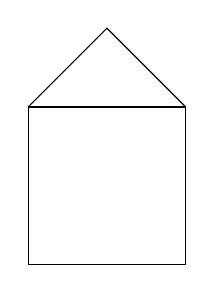
\begin{tikzpicture}

        % (x, y): x horizontal, y vertical; every instruction ends with ;
        % \draw (0, 0) -- (2, 0);
        % \draw (2, 0) -- (2, 2);
        % \draw (2, 2) -- (0, 2);
        % \draw (0, 2) -- (0, 0);

        \draw (0, 0) -- (2, 0) -- (2, 2) -- (0, 2) -- (0, 0);
        \draw (0, 2) -- (1, 3) -- (2, 2);
        %\draw (1, 3) -- (2, 2);

    \end{tikzpicture}
    \caption{Our first TikZ figure}
    \label{fig:first_tikz}
\end{figure}

\lipsum[3-4]

\end{document}
